Si inverte la matrice precedentemente ottenuta:
$$
\begin{bmatrix}
Q_1\\
Q_2
\end{bmatrix} = \frac{4\pi \varepsilon_0}{\frac{1}{R_1R_2}-\frac{1}{d^2}} \begin{bmatrix}
\frac{1}{R_2} & -\frac{1}{d}\\
-\frac{1}{d} & \frac{1}{R_1}
\end{bmatrix}\begin{bmatrix}
V_1 \\
V_2
\end{bmatrix}
$$
Si ottengono quindi le capacità parziali:
\begin{align*}
&C_{11} = \frac{4\pi\varepsilon_0}{\frac{1}{R_1R_2}-\frac{1}{d^2}}\frac{1}{R_2} & C_{12} = 
\frac{4\pi\varepsilon_0}{\frac{1}{R_1R_2}-\frac{1}{d^2}}\left(-\frac{1}{d}\right)\\
&C_{22} = \frac{4\pi\varepsilon_0}{\frac{1}{R_1R_2}-\frac{1}{d^2}}\frac{1}{R_1} & C_{21} = 
\frac{4\pi\varepsilon_0}{\frac{1}{R_1R_2}-\frac{1}{d^2}}\left(-\frac{1}{d}\right)
\end{align*}
\begin{align*}
&C_{11}^* = C_{11} + C_{12} = \frac{4\pi\varepsilon_0}{\frac{1}{R_1R_2}-\frac{1}{d^2}}
\left(\frac{1}{R_2} - \frac{1}{d}\right)\\
&C_{22}^* = \frac{4\pi\varepsilon_0}{\frac{1}{R_1R_2}-\frac{1}{d^2}}
\left(-\frac{1}{d} + \frac{1}{R_1}\right)\\
&C_{12}^* = -\frac{4 \pi \varepsilon_0}{\frac{1}{R_1R_2}-\frac{1}{d^2}}\left(-\frac{1}{d}\right) =
\frac{4 \pi \varepsilon_0}{\left(\frac{1}{R_1R_2} - \frac{1}{d^2}\right)}\cdot\frac{1}{d} = \frac{4\pi\varepsilon_0 R_1R_2d}{d^2-R_1R_2}
\end{align*}

Se supponiamo che ci sia un fenomeno di induzione completa: 
$$
Q_2 = -Q_1 \Rightarrow C = C_{12}^* +
\left(\frac{1}{C_{11}^*} + \frac{1}{C_{22}^*}\right)^{-1}
$$
$$
C = \frac{Q_1}{V_1-V_2} = \frac{1}{\frac{1}{4\pi\varepsilon_0}}\frac{Q_1}{\frac{Q_1}{R_1} -
\frac{Q_1}{d}-\left(\frac{Q_1}{d}-\frac{Q_1}{R_2}\right)} =
\frac{4\pi\varepsilon_0}{\frac{1}{R_1} + \frac{1}{R_2} - \frac{2}{d}}
$$
Eseguendo il limite per $d\to \infty$ si vede che l'espressione precedente è coerente con quella 
ricavata nell'ipotesi in cui le cariche siano poste a grande distanza.


\subparagraph{Capacità per unità di lunghezza di una linea bifilare}

I due conduttori possono essere rappresentati mediante due sezioni cilindriche,
le cariche associate $Q_1$ e $Q_2$ si accumuleranno per unità di lunghezza e 
saranno quindi misurate in \si{\coulomb\per\meter}.
Applicando il PSE
\begin{figure}[h!]
\centering
 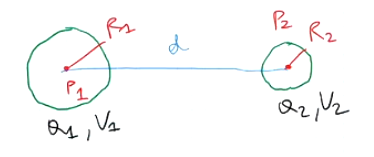
\includegraphics[width=0.5\linewidth]{conduttori_bifilari}
\caption{}
\end{figure} 

\begin{align*}
V_1' &= -\frac{\sigma_1 R_1}{\varepsilon_0} \ln R_1 & V_2' &= -\frac{\sigma_1 R_1}{\varepsilon_0} \ln d\\
V_1'' &= -\frac{\sigma_2 R_2}{\varepsilon_0} \ln d & V_2'' &= -\frac{\sigma_2 R_2}{\varepsilon_0} \ln R_2
\end{align*}
quindi moltiplicando e dividendo per $2\pi$
\begin{align*}
V_1 &= V_1' + V_1'' = -\frac{\sigma_1 2\pi R_1}{2\pi\varepsilon_0} \ln R_1 -\frac{\sigma_2 2\pi R_2}{2\pi\varepsilon_0} \ln d\\
V_2 &= V_2' + V_2'' = -\frac{\sigma_1 2\pi R_1}{2\pi\varepsilon_0} \ln d  -\frac{\sigma_2 2\pi R_2}{2\pi\varepsilon_0} \ln R_2
\end{align*}

Per ipotesi di induzione completa:
$$
C = \frac{Q_1}{V_1-V_2} = \frac{Q_1}{-\frac{Q_1}{2\pi\varepsilon_0}\ln R_1 + \frac{Q_2}{2\pi\varepsilon_0}\ln d + \frac{Q_1}{2\pi\varepsilon_0}\ln d - \frac{Q_2}{2 \pi \varepsilon_0} \ln R_2} = \frac{2\pi\varepsilon_0}{\ln \left(\frac{d^2}{R_1R_2}\right)}
$$

Se si suppone che i raggi dei conduttori siano gli stessi, come accade solitamente nelle linee multifilari, la capacità diventa
$$
C\cdot L = \frac{2\pi\varepsilon_0 L}{2 \ln \left(\frac{d}{R}\right)} = \frac{\pi \varepsilon_0 L}{\ln \left(\frac{d}{R}\right)} = 27.8\cdot 10^{-12} \frac{L}{\ln\left(\frac{d}{R}\right)}\ \ [\si{\farad}]
$$
Questa ipotesi è valida se non si considera l'influenza del suolo, per studiare l'effetto di questa 
presenza si usa il \textit{metodo delle immagini}.

\subparagraph{Realizzazione di un induttore con un condensatore}



\subsection{Materiali dielettrici}
E il loro modello elettromagnetico
